\chapter{Testing}
\label{cha:testing}
In this section the hardware and software tests performed are described on a
unit and integrated level.

\section{Software}
\label{sec:software}
In this section the software tests conducted over the \texttt{Remote Client},
\texttt{Remote Server}, \texttt{Database} and \texttt{Local System} are presented.

\subsection{Local System}
\label{sec:local-system}
The \texttt{Local system} tests were performed on a host computer, prior to its
deployment to the \texttt{Raspberry Pi}. These tests are described next.

\subsubsection{Computer vision}
\label{sec:computer-vision-1}
In this section are described the frame acquisition,
face detection, and gesture recognition tests. Fig.~\ref{fig:cv-tests}
illustrates the combination of these tests. It can be seen that the camera
frames are acquired and processed to detect multiple faces and apply filters overlay, and
also to detect gestures that can be used to trigger UI events.
Additionally, it can be seen a picture that was taken, stored and displayed,
which is ready for sharing on social media.
\begin{figure}[htb!]
\centering
    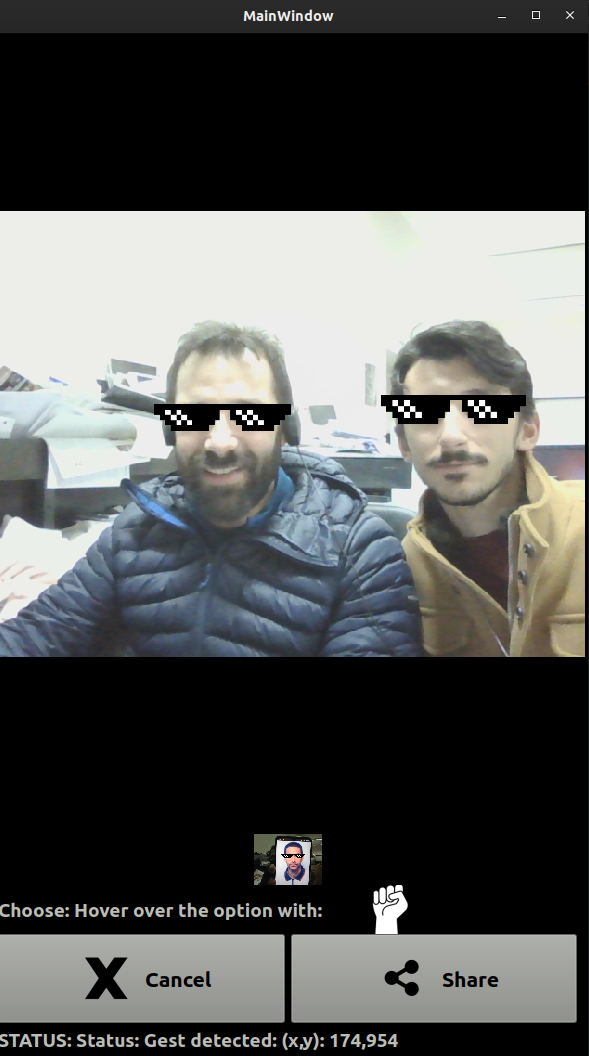
\includegraphics[width=0.6\textwidth]{./img/UI-test-filters.png}
  \caption{Computer visions tests}%
\label{fig:cv-tests}
\end{figure}

\subsubsection{Normal mode}
\label{sec:normal-mode}
Fig.~\ref{fig:normal-mode-test} illustrates the normal mode testing. It
demonstrated that a video can be reproduced on a loop while the fragrance
diffuser was also enabled and disabled according to its on and off times. The
normal mode only exited if there was no current ad enabled or if a user was
detected.
%
\begin{figure}[htb!]
\centering
    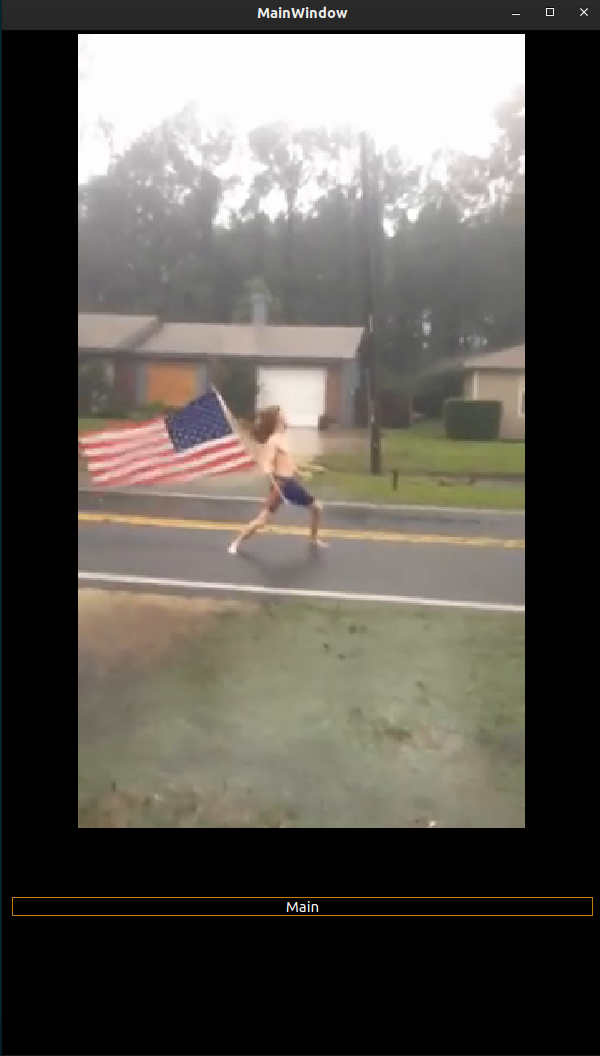
\includegraphics[width=0.6\textwidth]{./img/ui-test-normal-mode.png}
  \caption{Normal mode: testing}%
\label{fig:normal-mode-test}
\end{figure}

\subsubsection{Interaction mode}
\label{sec:interaction-mode}
The interaction mode tests demonstrated that it was possible to take pictures
and create GIFs on demand, as illustrated in Fig.~\ref{fig:cv-tests}.

\subsubsection{Twitter sharing}
\label{sec:twitter-sharing}
Fig.~\ref{fig:twitter-test} illustrates the Twitter sharing mode. It
demonstrated that a post can be successfully shared from the Local System into
Twitter. Nonetheless, at the current time, it is still not possible to upload
media to Twitter, as the API recently changed, requiring extra time to implement.
%
\begin{figure}[htb!]
  \centering
  % 
  \begin{subfigure}[t]{.4\textwidth}
  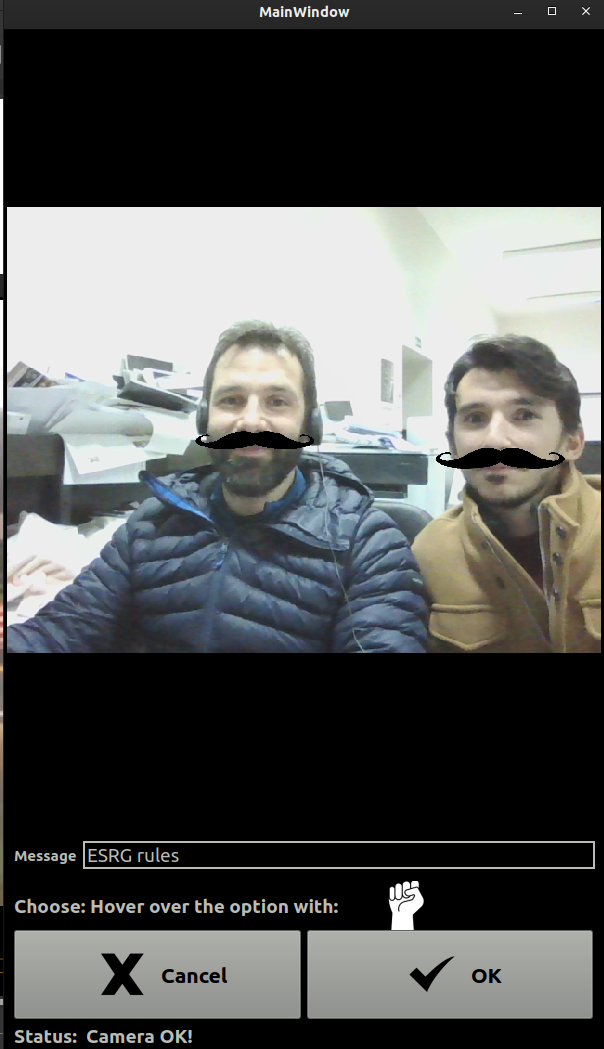
\includegraphics[width=\textwidth]{img/ui-test-sharing-mode.png}%
  %\caption{main}%
  %\label{fig:state-mach-local-superv-main}
\end{subfigure}
%
\hspace{.05\textwidth}
%
  \begin{subfigure}[t]{.42\textwidth}
  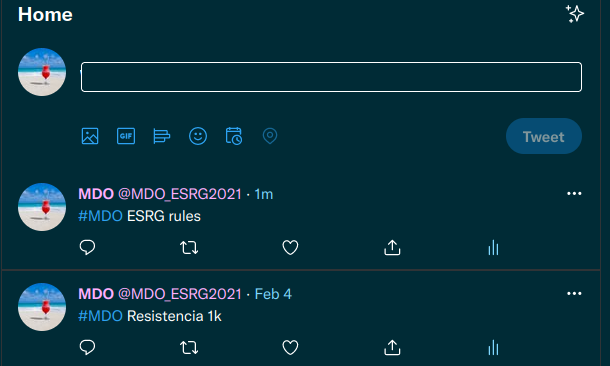
\includegraphics[width=\textwidth]{img/ui-test-sharing-mode2.png}%
  %\caption{Request Handler}%
  %\label{fig:state-mach-local-superv-req}
\end{subfigure}
  % 
  \caption{Twitter sharing: testing}%
  \label{fig:twitter-test}
\end{figure}
%

\subsubsection{Image filtering mode}
\label{sec:image-filtering-mode}
From Fig.~\ref{fig:cv-tests} and Fig.~\ref{fig:twitter-test}, it is possible to
verify that several filters were successfully implemented. Moreover, it is
possible to observe from the last figure that the image filter can be persistent
if desired.

\subsubsection{Download Ad}
\label{sec:download-ad}
Fig.~\ref{fig:download-test} illustrates the download of an Ad in the
background, while the application was currently busy in the interaction mode.
%
\begin{figure}[htb!]
\centering
    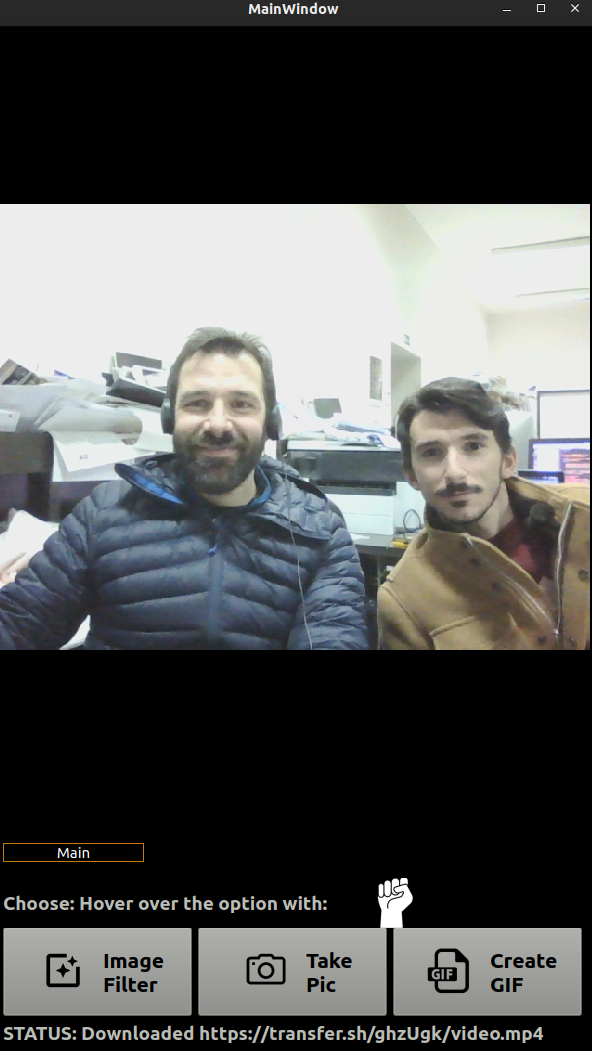
\includegraphics[width=0.6\textwidth]{./img/ui-test-download-ad.png}
  \caption{Download Ad: testing}%
\label{fig:download-test}
\end{figure}


\subsubsection{Connection to Remote System}
\label{sec:conn-remote-syst}
The connection to the remote system was simulated and tested deploying a server
listening in the \texttt{localhost} and observing the connection and data exchange between the two
nodes. This test was successful validating the client-server architecture logic
and implementation.

\subsubsection{User detection}
\label{sec:user-detection}
The user detection was tested by deploying the user detection daemon to
stimulate the application. It was verified that the daemon successfully detects
the ultrasonic sensors triggering when a person passes and that this event is
conveyed to the local system via message queue where it is successfully
detected, signaling a user was detected.

%%% Local Variables:
%%% mode: latex
%%% TeX-master: "../../../dissertation"
%%% End:
